\documentclass[11pt]{scrartcl}
\usepackage[sexy]{evan}
\usepackage{graphicx}
\graphicspath{ {./images/} }

\usepackage{answers}
\Newassociation{hint}{hintitem}{all-hints}
\renewcommand{\solutionextension}{out}
\renewenvironment{hintitem}[1]{\item[\bfseries #1.]}{}

\usepackage{venndiagram,multicol,hyperref,graphicx,array}

\begin{document}
\title{Principio de Casillas}
\author{Ricardo Largaespada}
\date{20 Abril 2024}

\maketitle
\section{Introducción}
Principio del Palomar también es conocido en algunos países (como en Rusia, por ejemplo) como el Principio de Dirichlet, ya que fue el matemático Lejeune Dirichlet el primero en utilizar este método para resolver problemas no triviales. Otros matemáticos que se destacaron por usar esta idea para resolver diversos problemas fueron los húngaros Erdős y Szekeres. Abordaremos este principio de la siguiente manera:\\

``Si en $n$ cajas se colocan $n + 1$ palomos, entonces al menos una caja tendrá más de un palomo.''\\

Algunos ejemplos:\begin{itemize}
\item[i.] En un grupo de tres personas, al menos dos de ellas son del mismo sexo.
\item[ii.] En un grupo de 13 personas, al menos dos de ellas tienen el mismo signo.
\item[iii.] En un grupo de 5 cartas de baraja, al menos dos son del mismo palo.
\item[iv.] En la ciudad de Managua, hay al menos dos personas con el mismo número de cabellos.
\end{itemize}
Ahora veamos cómo algo tan simple puede resolver problemas aparentemente difíciles:

\begin{example}
Se eligen 5 puntos al azar sobre la superficie de un cuadrado de lado 2. Demuestra que al menos dos de estos puntos están a una distancia menor o igual a $\sqrt2$.
\end{example}
Solución. Dividimos el cuadrado en cuatro cuadrados más pequeños como se muestra en la figura adjunta. Como tenemos cinco puntos y cuatro cuadrados, tendremos al menos dos puntos en el mismo cuadradito. Como la mayor distancia entre dos puntos del mismo cuadradito no supera la medida de su diagonal, el resultado sigue inmediatamente.

\begin{center}
    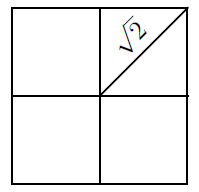
\includegraphics[scale=1]{images/clase_07_sqrt2.png}
\end{center}

\section{¿Paso Mágico?}
Para el alumno principiante, la solución del problema anterior puede haber parecido un poco mágica. Vamos a mostrar que no es exactamente así, que existe un método en la resolución de algunos problemas simples que utilizan la idea del palomar. La primera cosa que debemos aprender a reconocer es cuándo un problema se trata de un problema sobre casillas. Esto puede adquirirse con experiencia, pero vamos a dar un pequeño empujón. Un problema de PC (Principio de las Casillas) tiene casi siempre la siguiente forma:\\

Dado un conjunto de \(n\) objetos, demuestra que podemos elegir \(k\) de ellos satisfaciendo una propiedad.\\

Bueno, después de identificar que el enunciado del problema no sugiere la idea de utilizar PC, debemos concentrarnos en responder las siguientes preguntas:
\begin{itemize}
\item[(i)] ¿Quiénes son las palomas?
\item[(ii)] ¿Cuántas son los palomares?
\item[(iii)] ¿Quiénes son los palomares?
\end{itemize}
Casi siempre, las dos primeras preguntas son las más fáciles de responder. Para responder a la tercera pregunta, debemos pensar en el concepto dual del espacio muestral. Por un lado, el espacio muestral es el conjunto de las posibles posiciones de los palomos. Por otro lado, es la unión de todas las casas.
Para finalizar, debemos dividir el espacio muestral en el número de casas ya descubierto. En este momento, es importante recordar que las casillas deben reflejar la propiedad deseada. Como acabamos de ver, utilizar el principio del palomar no es difícil. Lo difícil está en encontrar quiénes serán nuestros "palomas" y "palomares". El próximo problema es, en principio, un problema de teoría de números. Sin embargo, vamos a utilizar el principio de casillas para resolverlo.

\begin{example}
    Demuestra que dados siete enteros positivos, existen dos cuya suma o diferencia es un múltiplo de 10.
\end{example}
Solución. Vamos a organizar seis cajas \(C_0, C_2, \ldots, C_5\) donde un entero está en la caja \(C_i\) si es congruente a \(i\) o a \(-i\) módulo 10. Sabemos que habrá dos enteros en la misma caja. De esta forma, si son incongruentes módulo 10, basta sumarlos. En caso contrario, toma su diferencia.

\begin{example}
Dados 5 puntos en el plano con coordenadas enteras, demuestra que al menos uno de los diez puntos medios generados por ellos también tiene coordenadas enteras.    
\end{example}
Solución. Podemos dividir los puntos de coordenadas enteras (representado como \(\mathbb{Z} \times \mathbb{Z}\)) en cuatro grupos \(G_1, G_2, G_3, G_4\) de la siguiente manera:\begin{itemize}
\item[i)] \(G_1 = \{(x, y) \in \mathbb{Z} \times \mathbb{Z} \mid x, y\) son ambos pares\}.
\item[ii)] \(G_2 = \{(x, y) \in \mathbb{Z} \times \mathbb{Z} \mid x, y\) son ambos impares\}.
\item[iii)] \(G_3 = \{(x, y) \in \mathbb{Z} \times \mathbb{Z} \mid x\) es par y \(y\) es impar\}.
\item[iv)] \(G_4 = \{(x, y) \in \mathbb{Z} \times \mathbb{Z} \mid x\) es impar y \(y\) es par\}.
\end{itemize}
Observa que los puntos que pertenecen al mismo grupo tienen puntos medios con coordenadas enteras. Como tenemos 5 puntos, el principio de casillas nos garantiza que hay al menos dos puntos en el mismo grupo.

\begin{example}
Nueve puntos se colocan sobre la superficie de un tetraedro regular con 1 cm de arista. Demuestra que entre estos puntos es posible encontrar dos con una distancia (espacial) no mayor que 0.5 cm.
\end{example}
Solución. Vamos a dividir la superficie del tetraedro en 16 triángulos equiláteros congruentes, dividiendo cada cara en cuatro partes usando sus bases medias. Ahora creamos 8 regiones coloreando estos triángulos según la siguiente regla: los triángulos que comparten un mismo vértice del tetraedro serán coloreados del mismo color; de esta forma ya hemos usado cuatro colores diferentes para 12 triángulos y los otros cuatro los pintaremos usando los colores restantes. De acuerdo con el principio de casillas, al menos dos de los nueve puntos estarán en la misma región. Solo falta notar que la distancia máxima entre dos puntos de la misma región es a lo sumo 0.5 cm.
\begin{center}
    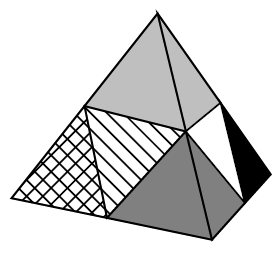
\includegraphics[scale=1]{images/clase_07_tetraedro.png}
\end{center}

\Opensolutionfile{all-hints}

\section{Problemas Propuestos}
\begin{problem}
Cincuenta y un puntos son colocados en el interior de un cuadrado de lado 1 metro. Demuestra que existe un conjunto de tres de estos puntos que pueden ser cubiertos por un cuadrado de lado 20 centímetros.
\begin{hint}
Imita la solución del problema 1.
\end{hint}
\end{problem}

\begin{problem}
En cada casa de un tablero 3 $\times$ 3 se coloca uno de los números $-1$, $0$, $1$. Demuestra que entre las ocho sumas a lo largo de una misma fila, columna o diagonal, hay dos iguales.
\begin{hint}
La suma de tres números varía en el conjunto \(\{-3, -2, -1, 0, 1, 2, 3\}\), como hay 8 sumas, al menos una será utilizada más de una vez.
\end{hint}
\end{problem}

\begin{problem}
Demuestra que de cualquier conjunto de diez enteros podemos elegir un subconjunto cuya suma es un múltiplo de 10.
\begin{hint}
Si \(a_1, a_2, \ldots, a_{10}\) son los números, considera las sumas
\begin{align*}
S_1 &= a_1 \\
S_2 &= a_1 + a_2 \\
S_3 &= a_1 + a_2 + a_3 \\
\ldots \\
S_{10} &= a_1 + a_2 + \ldots + a_{10}.
\end{align*}
Si una de ellas es un múltiplo de 10, habremos encontrado la solución del problema. De lo contrario, como hay 9 restos posibles (diferentes de cero) en la división por 10, por el PC, existirán dos de estas sumas que serán congruentes módulo 10. Si \(S_i \equiv S_j \pmod{10}\), entonces
\[ S_i - S_j \equiv a_i + a_{i+1} + \ldots + a_j \equiv 0 \pmod{10}. \]
Esto concluye la solución.
\end{hint}
\end{problem}

\begin{problem}
Demuestra que existe una potencia de 3 terminada en los dígitos 001 (en base decimal).
\begin{hint}
Utiliza el PC para demostrar que existen dos potencias de 3 con el mismo resto en la división por 1000.
\end{hint}
\end{problem}

\begin{problem}
Muestra que un triángulo equilátero no puede ser totalmente cubierto por otros dos triángulos equiláteros más pequeños.
\begin{hint}
Observa lo que sucede en los vértices del triángulo mayor.
\end{hint}
\end{problem}

\begin{problem}[Longlist IMO 1977] Dados 37 puntos en el espacio con coordenadas enteras, demuestra que al menos uno de los triángulos formados por tres de estos puntos tiene el baricentro con coordenadas enteras.
\begin{hint}
Adapta la solución del problema 3.
\end{hint}
\end{problem}

\begin{problem}[Bielorrusia 1996] En un grupo de 29 hobbits, algunos de ellos dicen la verdad y otros siempre mienten. En un cierto día de primavera, todos se sentaron alrededor de una mesa, y cada uno de ellos dijo que sus dos vecinos eran mentirosos.
\begin{itemize}
    \item[a)] Demuestra que al menos 10 hobbits dicen la verdad.
    \item[b)] ¿Es posible que exactamente 10 de ellos digan la verdad?
\end{itemize}
\end{problem}

\begin{problem}
En cada casa de un tablero 10 $\times$ 10 se coloca un entero de modo que la diferencia positiva entre los enteros de dos casas vecinas (lado en común) sea como máximo 5. Demuestra que dos de estos enteros deben ser iguales.
\end{problem}

\begin{problem}
Treinta y tres torres se colocan en un tablero 8 $\times$ 8. Demuestra que podemos elegir cinco de ellas sin que ninguna ataque a otra.
\begin{hint}
Pinta el tablero usando 8 colores como en el siguiente diagrama:
\[
\begin{matrix}
1 & 2 & 3 & 4 & 5 & 6 & 7 & 8 \\
2 & 3 & 4 & 5 & 6 & 7 & 8 & 1 \\
3 & 4 & 5 & 6 & 7 & 8 & 1 & 2 \\
4 & 5 & 6 & 7 & 8 & 1 & 2 & 3 \\
5 & 6 & 7 & 8 & 1 & 2 & 3 & 4 \\
6 & 7 & 8 & 1 & 2 & 3 & 4 & 5 \\
7 & 8 & 1 & 2 & 3 & 4 & 5 & 6 \\
8 & 1 & 2 & 3 & 4 & 5 & 6 & 7 \\
\end{matrix}
\]
Por el PC, habrá al menos 5 torres en casillas del mismo color. Observa que las torres en casillas del mismo color no se atacan.
\end{hint}
\end{problem}

\begin{problem}[Longlist IMO 1979] Colocamos $4n + 1$ reyes en un tablero infinito. Demuestra que podemos elegir $n + 1$ de ellos de modo que no existan dos que se ataquen.
\begin{hint}
Pinta el tablero usando 4 colores como en el siguiente diagrama:
\[
\begin{matrix}
1 & 2 & 3 & 4 & 1 & 2 & 3 & 4 \\
2 & 3 & 4 & 1 & 2 & 3 & 4 & 1 \\
3 & 4 & 1 & 2 & 3 & 4 & 1 & 2 \\
4 & 1 & 2 & 3 & 4 & 1 & 2 & 3 \\
\end{matrix}
\]
Repite el argumento anterior.
\end{hint}
\end{problem}

\begin{problem}
Demuestra que de cualquier subconjunto de $n + 1$ elementos del conjunto $\{1, 2, \ldots, 2n\}$ es posible elegir dos que sean primos entre sí.
\begin{hint}
Separa el conjunto en \(n\) pares de elementos consecutivos.
\end{hint}
\end{problem}

\begin{problem}[IMO 1972] Demuestra que, de cualquier conjunto de diez números distintos de dos dígitos, podemos elegir dos subconjuntos $A$ y $B$ (disjuntos) cuya suma de los elementos es la misma en ambos.
\end{problem}

\begin{problem}
Cuarenta estudiantes participaron en una olimpiada de matemáticas. La prueba consistió en cinco problemas en total. Se sabe que cada problema fue resuelto correctamente por al menos 23 participantes. Demuestra que debe haber dos participantes tales que todos los problemas fueron resueltos por al menos uno de ellos dos.
\end{problem}

\begin{problem}
    Demuestra que en cualquier grupo de 17 números elegidos del conjunto $M = \{1, 2, 3, \ldots, 24, 25\}$ es posible elegir dos cuyo producto es un cuadrado perfecto.
\end{problem}
\Closesolutionfile{all-hints}

\section{Sugerencias y Soluciones}
\begin{enumerate}
\input{all-hints.out}
\end{enumerate}

\end{document}